\documentclass[../MATLAB_Primer.tex]{subfiles}
\begin{document}
\subsection{MATLAB Layout} \label{MATLAB Layout}
The MATLAB application has four key layout components: The Command Window, the Workspace, the Editor (or Live Editor), and the Current Folder. If any of these components do not appear in your MATLAB application, you can go to the Home tab, and in the Environment section, click layout. Here you can toggle the layout components on or off.
\\ \\
In Figure \ref{fig:matlabLayout} below you can see that the Live Editor takes up the majority of the space in the center, the Workspace is on the right, the Command Window is on the bottom, and the Current Folder is on the left. However, the MATLAB layout can be customized and does not require these placements. To customize the interface to match your personal preferences, you may drag and drop components to different sections of the interface.
\begin{figure}[h]
    \centering
    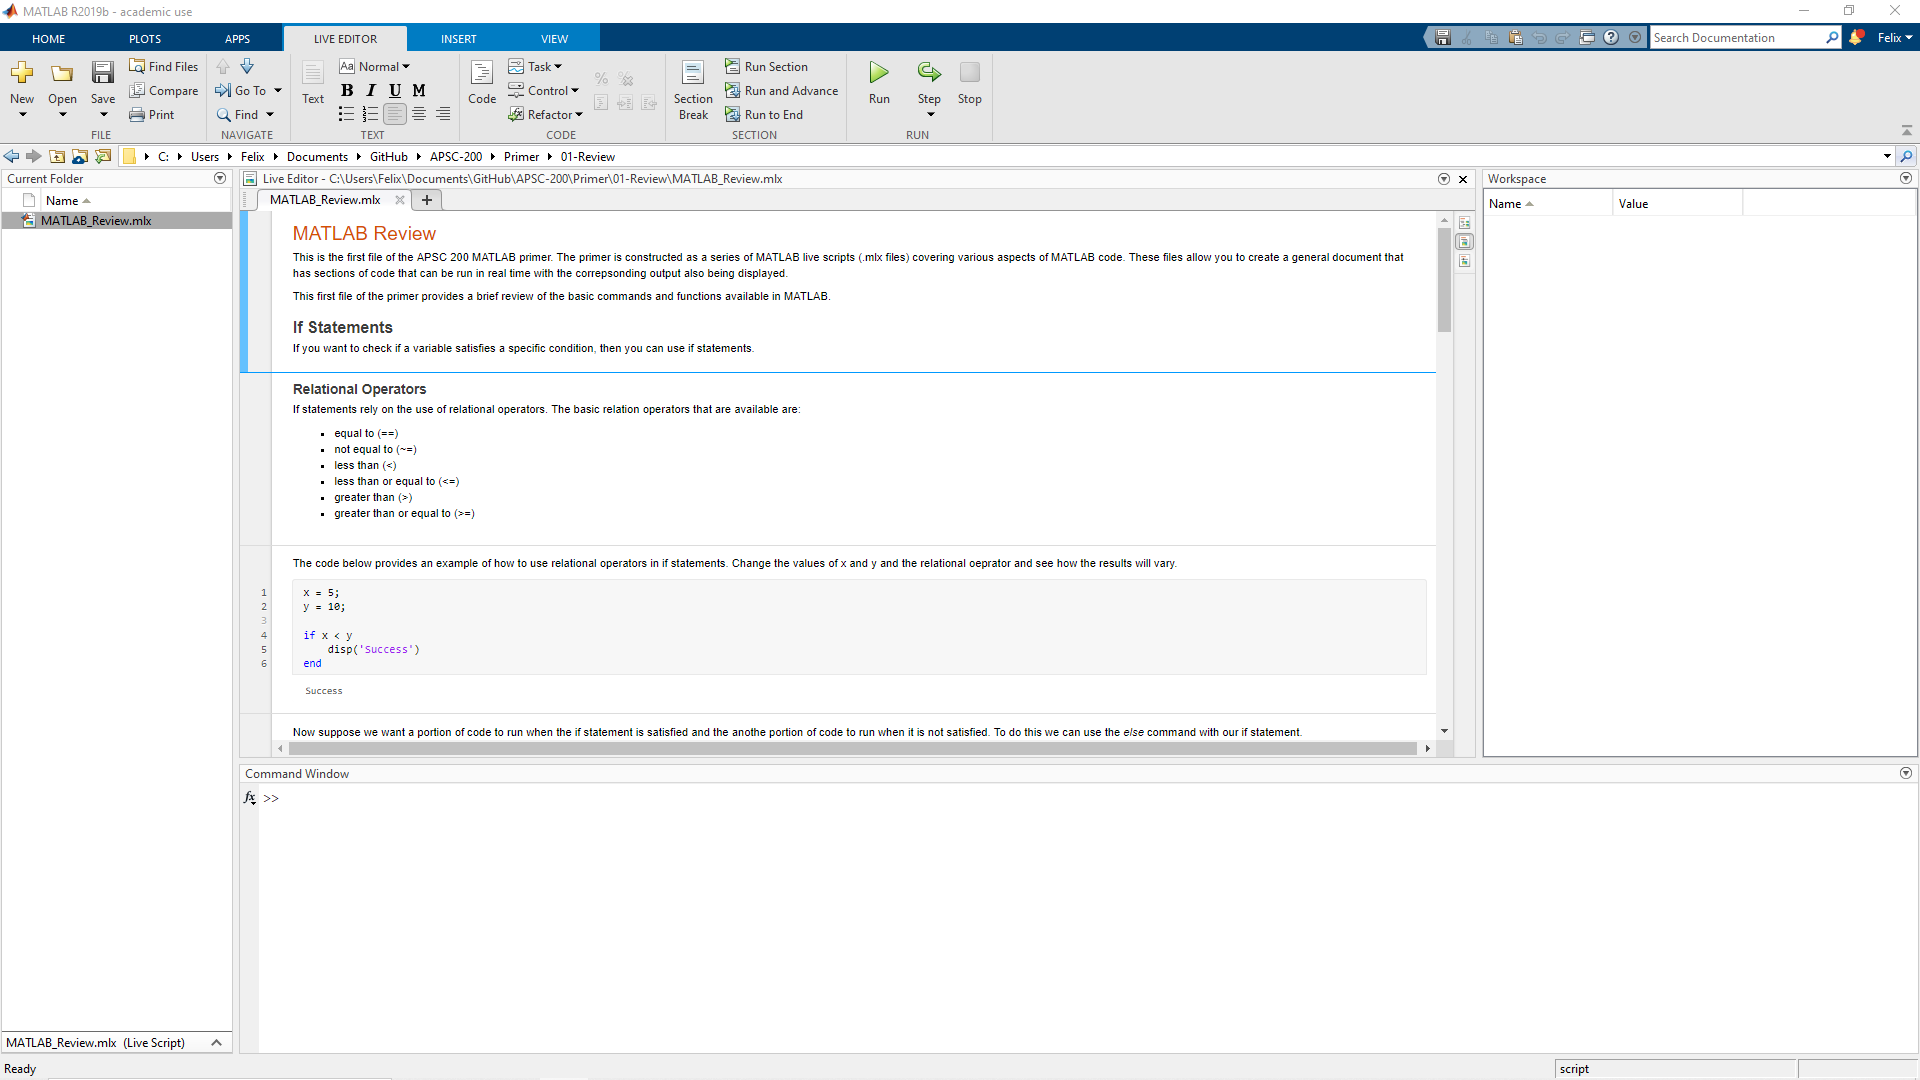
\includegraphics[width=426pt]{images/matlabLayout.PNG}
    \caption{MATLAB Layout}
    \label{fig:matlabLayout}
\end{figure}

\subsubsection{Command Window}
MATLAB's Command Window enables you to write single-line input statements and view corresponding output statements. Input statements written in the Command Window will result in an output statement being displayed below them; however, output statements can be suppressed through the use of a semi-colon at the end of a command.
\\ \\
Example 1:
\\ \\
\textit{input:}
\begin{lstlisting}[frame=single]
>> 1 + 1 % this command will appear as an output
\end{lstlisting}

\textit{output:}

\begin{center}
    ans = 2
\end{center}

Example 2:
\\ \\
\textit{input:}
\begin{lstlisting}[frame=single]
>> 2 + 2; % this command will not appear as an output
\end{lstlisting}

\textit{output:}

\begin{center}
    
\end{center}

There are a number of functions you can use to print variables to the Command Window. Removing the semi-colon at the end of specific line of code that you want displayed is considered to be poor practice. Instead you can use the \texttt{disp()} function within MATLAB to print your variable.
\\ \\
Example:
\\ \\
\textit{input:}
\begin{lstlisting}[frame=single]
>> x = 10;
>> disp(x)
\end{lstlisting}

\textit{output:}

\begin{center}
    10
\end{center}

If you want to create a string that contains a variable, you can use the \texttt{sprintf()} function. This function allows you to specify formatting such as how many decimal places of the variable should be shown in the string. The string can then be displayed using the \texttt{disp()} function.
\\ \\
Example 1:
\\ \\
\%d is used within a string to represent an integer (x) which is entered as the second argument in the \texttt{sprintf()} function after the string.
\\ \\
\textit{input:}
\begin{lstlisting}[frame=single]
>> output1 = sprintf('There are %d agents.', x); 
>> disp(output1);
\end{lstlisting}

\textit{output:}

\begin{center}
    There are 10 agents.
\end{center}

Example 2:
\\ \\
\%f is used within a string to represent a floating point number (y) which is entered as the second argument in the \texttt{sprintf()} function after the string. The .2 specifies that the floating point number should be rounded to two decimal places.
\\ \\
\textit{input:}
\begin{lstlisting}[frame=single]
>> y = 12.1250;
>> output2 = sprintf('The value of y is: %.2f', y); 
>> disp(output2);
\end{lstlisting}

\textit{output:}

\begin{center}
    The value of y is: 12.13
\end{center}

Additionally, MATLAB has the \texttt{fprintf()} function which combines \texttt{disp()} and \texttt{sprintf()}. \texttt{fprintf()} takes a string a variables as inputs similar to \texttt{sprintf()}, and displays the string as output. It is common practice to end the string input with the new line character \texttt{\textbackslash n} to ensure a new line is printed after the string. \\ \\
Example 3:
\\ \\
\%f is used within a string to represent a floating point number (z) which is entered as the second argument in the \texttt{sprintf()} function after the string. The .0 specifies that the floating point number should be rounded to the nearest integer.
\\ \\
\textit{input:}
\begin{lstlisting}[frame=single]
>> z = 9.5;
>> fprintf('The value of z is: %.0f\n', z); 
\end{lstlisting}

\textit{output:}

\begin{center}
    The value of z is: 10
\end{center}

As the Command Window processes single-line input statements one at a time, it is not possible to edit statements that have already been ran; however, you can navigate through and run previously ran statements using the up and down arrow keys. Additionally, you can navigate through and run a series of previously ran statements by holding down the shift key while using the up and down arrow keys.
\\ \\
Furthermore, you can clear all previously inputted statements with the following command:
\\ \\
\textit{input:}
\begin{lstlisting}[frame=single]
>> clc % this command will clear the Command Window
\end{lstlisting}

\begin{center}
    
\end{center}

\subsubsection{Workspace}
MATLAB's Workspace is used to store and display variables. Variables can be created via declaration statements, or they can be imported from data files (.mat) via \texttt{load} statements. Additionally, variables stored in the Workspace can be exported to data files via \texttt{save} statements.
\\ \\
Example 1:
\\ \\
\textit{input:}
\begin{lstlisting}[frame=single]
>> x = 5; % x will be stored in the workspace with a value of 5
\end{lstlisting}

\textit{output:}

\begin{center}
    
\end{center}
Example 2:
\\ \\
\textit{input:}
\begin{lstlisting}[frame=single]
>> load data.mat; % variables in data.mat will be loaded into the Workspace
\end{lstlisting}
\textit{output:}

\begin{center}
    
\end{center}
Example 3:
\\ \\
\textit{input:}
\begin{lstlisting}[frame=single]
>> save mydata.mat; % variables in the Workspace will be saved in mydata.mat
\end{lstlisting}

\textit{output:}

\begin{center}
    
\end{center}
Furthermore, you can clear the Workspace with the following command:
\\ \\
\textit{input:}
\begin{lstlisting}[frame=single]
>> clear % this command will clear the Workspace
\end{lstlisting}

\textit{output:}

\begin{center}
    
\end{center}

\subsubsection{Editor (or Live Editor)}
MATLAB's Editor and Live Editor components are used for writing scripts (.m files) and live scripts (.mlx files), respectively. The Editor enables you to write multi-line input statements to be processed sequentially. When running scripts, outputs will appear in the Command Window. When running live scripts, outputs will appear beside or beneath your code within the Live Editor.

\subsubsection{Current Folder}
MATLAB's Current Folder section enables you to view which directory you are working out of. Typically, you will want to write scripts that are able to call functions and load data from other files. To do so, you should understand how to effectively manage files and folders in MATLAB.  A common issue that arises for new programmers is that a file needed in a script (e.g. a .csv file) is not located in the current directory where the script itself is located.  
\\ \\
Useful functions:
\\ \\
\textit{input:}
\begin{lstlisting}[frame=single]
>> currentFolder = pwd % used to print the working directory
\end{lstlisting}

\textit{output:}

\begin{center}
    currentFolder = 'C:\textbackslash Users\textbackslash Felix\textbackslash Documents\textbackslash GitHub\textbackslash APSC-200\textbackslash Primer\textbackslash 01-Review'
\end{center}

\textit{input:}
\begin{lstlisting}[frame=single]
>> cd 'C:\Users\Felix\Documents\GitHub\APSC-200\Primer\02-ArraysMatrices' 
% used to change the directory to a different folder
\end{lstlisting}

\textit{output:}

\begin{center}
    
\end{center}

\textit{input:}
\begin{lstlisting}[frame=single]
>> currentFolderContents = ls 
% used to list folder contents of the current directory
\end{lstlisting}

\textit{output:}

\begin{center}
    currentFolderContents =\\
    '.                  '\\
    '..                 '\\
    'CellArrays.mlx     '\\
    'Intro.mlx          '\\
    'LogicalIndexing.mlx'\\
\end{center}
Note the first two items of the array, '.' and '..'. These entries correspond to the current folder and the parent folder, respectively. Hence, if I wanted to change to the parent directory, I could enter:
\\ \\
\textit{input:}
\begin{lstlisting}[frame=single]
>> currentFolderContents = cd .. 
% used to change the directory to the parent folder
\end{lstlisting}

\textit{output:}

\begin{center}
    
\end{center}

\subsubsection{Search Documentation}
    Lastly, one other key component of the MATLAB interface that you will likely use often is the Search Documentation bar that can be found in the upper right corner of the interface. The Search Documentation bar will allow you to find syntax, descriptions, and examples of all MATLAB functions and it should be your first point of contact when seeking to understand and utilize new functions.
    
\end{document}